\documentclass[10]{article}
\usepackage[margin=1in]{geometry}

\usepackage{graphicx}
\graphicspath{{../../data/features/visualize/}}
\usepackage{fancyvrb,color,amssymb,float,alltt,verbatim}
\usepackage{amsmath,mathtools,listings,multicol,hyperref,enumerate}
\usepackage[usenames,dvipsnames,svgnames,table,hyperref]{xcolor}

\usepackage{color}
\usepackage[backend=biber]{biblatex}
\bibliography{milestone}

\begin{document}
\begin{center}
\huge{\textbf{CS229 - Milestone Report}} \\
\end{center}
\begin{center}
\normalsize{11 13 2015} \\

Keri A. McKiernan \\
Joe Napoli
\end{center}
%------------------------------------------------------------------------------%
\section*{Introduction and Methods}
Public interest has become increasingly concentrated on the effect of money in politics. Specifically, the Citizens United v. FEC Supreme Court ruling maintained the legality of unrestricted political expenditures by corporate and union entities. As a result, there has been a proliferation of super PAC, or `political action committee',  organizations. While these organizations are not permitted to make contributions directly to candidates’ campaigns, they may engage in unlimited independent spending and there is no restriction on the amount of funds they can accept from donors. These legal developments beg the question: Can one predict explicitly the influence of donors over politicians to whom they give? \\

The research of Poole and Rosenthal has focused on quantifying the political ideology of politicians \cite{PR}. In particular, they actively develop methods for calculating "ideal points" for candidates. The DW-NOMINATE method calculates a legislator’s overall probability of voting "yea" on an item of legislation as the sum of a deterministic utility value and a random error \cite{NOMBOOT}. "Ideal point" coordinates were obtained for legislators by maximizing the log likelihood function

\[ \sum_{t=1}^{T} \sum_{i=1}^{p_t} \sum_{j=1}^{q_t} \sum_{\tau = 1}^{2} C_{ij \tau t} \ln P_{ij \tau t} \]

\noindent where $P_{ij \tau t}$ is the probability of voting for choice $\tau$ (yes or no) and $C_{ij \tau t} = 1$ if that probability accurately predicts the vote \cite{NOMBOOT}. Indexes $j$, $i$, and $t$ sum over roll call votes, legislators, and legislative sessions, respectively. Ideal points are constrained to lie within the interval $\left[ -1,1 \right]$ and are two-dimensional quantities. A common interpretation of the first coordinate is that it reflects the divide between the Republican and Democratic parties, whereas the second coordinate is more highly correlated with intra-party division. While a full congressional voting record is not available for candidates who are new to office, campaign finance data is readily available. It would be useful to be able to predict the ideal point of a candidate even before they have established a congressional voting record. Furthermore, the ability to do so would help elucidate a relationship between monetary contributions to candidates and the voting patterns those contributions may effect.\\

We have collated freely available campaign finance and DW-NOMINATE ideal point \cite{DWWEB} datasets and performed a principal component analysis on the feature set extracted therefrom. The original scope of our project has been narrowed due to a reduction in the size of our group. While originally we had planned to investigate anomalous voting behavior and the ability to predict it solely by examining campaign finance data, we have shifted our focus on training a model to predict DW-NOMINATE ideal points, which directly reflect ideological stances and inter-/intra-party divisions. This shift has been prompted by datasets that were relatively more sparse than expected as well as the challenge of collating them.\\

\section*{PCA of Features}
Financial data for a set of moderate candidates (as determined by sampling from the DW-NOMINATE scores) was obtained using the Open Secrets python API.  Of the available data, we chose to partition finance streams by sector.  For each sector, individual and PAC contributions are available.  These values were normalized separately as, in some cases, the relative magnitudes were very large.  Useful normalization of these vectors (weight determination) remains a future direction for this project.  These results can be seen in figure \ref{fig:fmtrx}.

\begin{figure}[H]
\centering
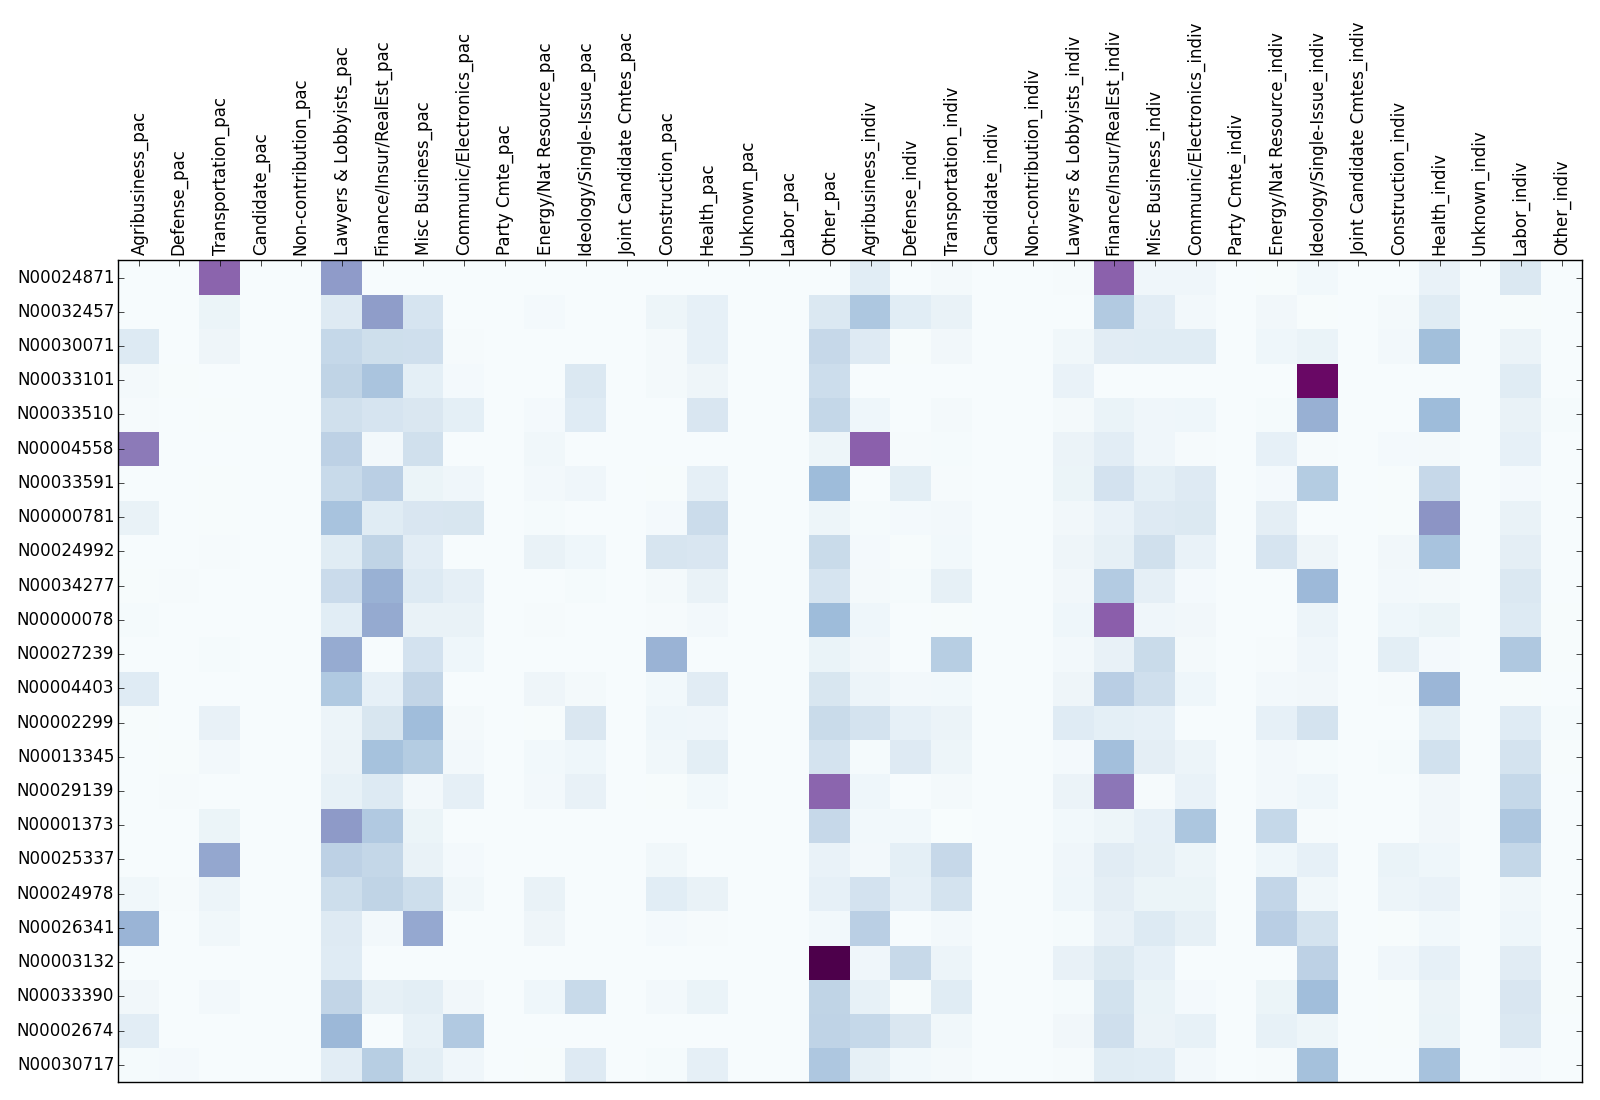
\includegraphics[width=.9\textwidth]{../../data/features/visualize/features.png}
\caption{\label{fig:fmtrx}Heatmap of feature matrix.}
\end{figure}
PCA was run on this feature matrix under a variety of conditions.  The `Other' category was first removed, as it is nondescript and lead to skewed results.  Then, the top 5 principal components  (without `Other') were calculated on the full matrix, PAC contributions only, and individual contributions only.
\begin{figure}[H]
\centering
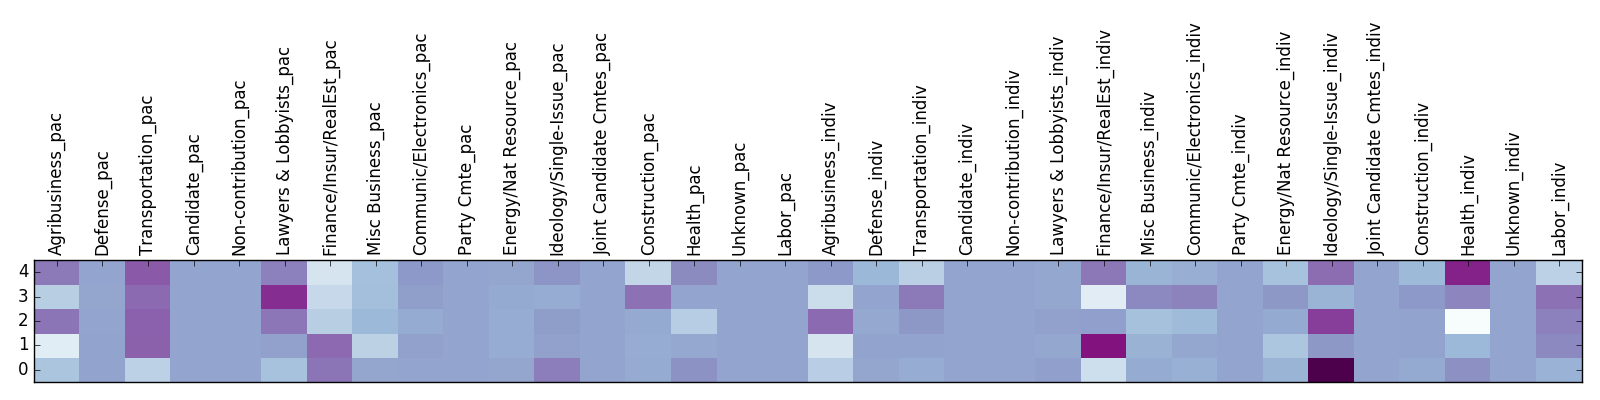
\includegraphics[width=.9\textwidth]{../../data/features/visualize/pcs_no_other.png}
\caption{\label{fig:pc_all}Heatmap of PCA eigenvectors of feature matrix without `Other'.}
\end{figure}
\begin{figure}[H]
\centering
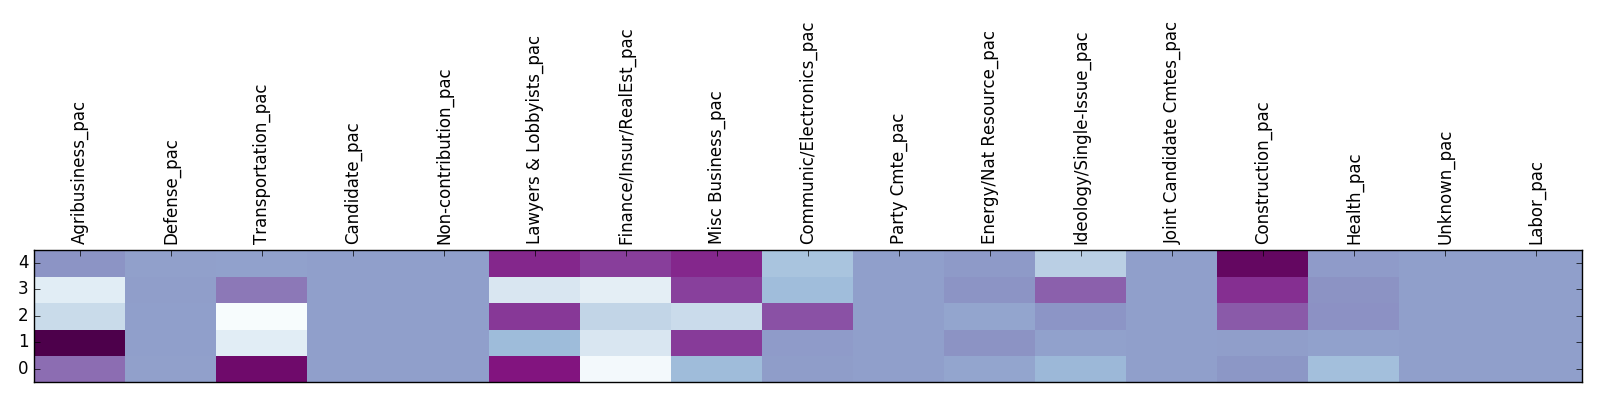
\includegraphics[width=.9\textwidth]{../../data/features/visualize/pcs_no_other_pac.png}
\caption{\label{fig:pc_all}Heatmap of PCA eigenvectors of PAC feature matrix without `Other'.}
\end{figure}
\begin{figure}[H]
\centering
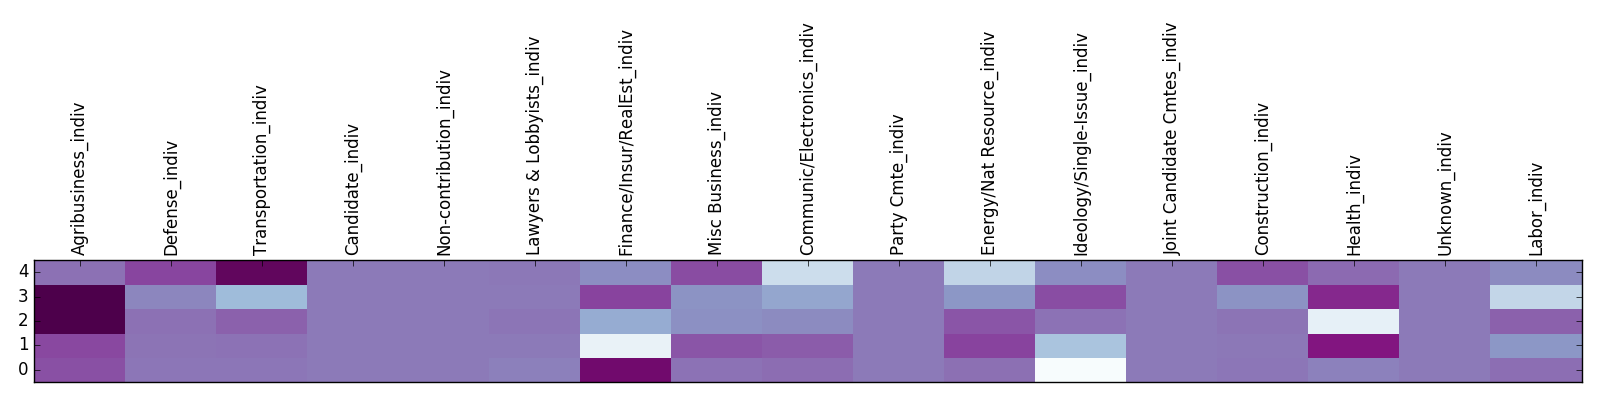
\includegraphics[width=.9\textwidth]{../../data/features/visualize/pcs_no_other_indiv.png}
\caption{\label{fig:pc_indiv}Heatmap of PCA eigenvectors of individual feature matrix without `Other'.}
\end{figure}
We see that there are several low variance components for both individial and PAC contributions: Defense, Candidate, Party Cmte, Joint Candidate Cmtes, and Unknown.  We could likely remove these values from our feature set when fitting a model.  The starkest difference between the PCs are in the Lawyers \& Lobbyists (high PAC variance, low individual variance) and Labor categories (low PAC variance, high individual variance).  These features may require special attention during model training. \\

Armed with a refined feature set and tools to query these features, we aim to train a model to predict DW-NOMINATE scores.  We plan to use a supervised learning method, starting with linear regression.  The results of this model will help us determine whether we will need to try a more sophisticated training algorithm.  We also plan to relay with our mentor about our approach so far and our planned future directions. 

\printbibliography

\end{document}
